\documentclass[12pt, letterpaper, twoside]{article}
\usepackage[utf8]{inputenc}
\usepackage[a4paper]{geometry}
\usepackage{array}
\usepackage{booktabs} % For prettier tables
\usepackage{multirow}
\usepackage{multicol}
\usepackage{ragged2e}
\usepackage{xcolor}
\usepackage{gensymb}
\usepackage{fullpage}
\usepackage{hyperref}
\usepackage{amsmath}
\usepackage{scrextend}
\usepackage{graphicx}

\graphicspath{ {./bilder/} }

\title{Bac 2014 Uppgift A1}
\author{Simon Freiermuth \\ \href{mailto:simon@freiermuth.org}{simon@freiermuth.org}}
\date{16 April, 2020}

\begin{document}

\begin{titlepage}
\maketitle
\end{titlepage}

\begin{flushleft}

%%%%%%%%%%%%%%%%%%%%%%%%%%%%%%%%%%%%%%%%%%%%%%%%%%%%%%%%%%%%%%%%%%%%%%%%%
% Begin
%%%%%%%%%%%%%%%%%%%%%%%%%%%%%%%%%%%%%%%%%%%%%%%%%%%%%%%%%%%%%%%%%%%%%%%%%
\begin{itemize}
%
\item[\textbf{a)}]En \textbf{stark} enprotonig syra $ HX $, är i fast form vid $ 25\ \degree C $.
Syran är den enda sura beståndsdelen i ett avkalkningsmedel för kaffemaskiner.

Antag att kalkavlagringarna i kaffemaskinen består av $ CaCO_3(s) $,
och ange ekvationen för reaktionen som kan observeras när avkalkaren gör sitt jobb.
\newline
\newline
$ CaCO_3(s)\ \overset{H_2O}{\rightarrow}\ Ca^{2+}(aq)\ +\ CO_3^{2-}(aq) $

$ 2HX(aq)\ +\ CaCO_3(s)\ \rightarrow\ H_2CO_3\ +\ Ca^{2+} + 2X^- $
\newline
%%%%%%%%%%%%%%%%%%%%%%%%%%%%%%%%%%%%%%%%%%%%%%%%%%%%%%%%%%%%%%%%%%%%%%%%%%
\item[\textbf{b)}]En kommersiell avkalkningsprodukt innehåller 91.0\%\ $ HX $ (massprocent).

För att kunna bestämma molmassan löser man upp $ 3.00\ g $ av avkalkaren i $ 5.00*10^{-1}\ dm^3 $ destillerat vatten.
Ett prov på $ 20.0\ cm^3 $ titreras med en natriumhydroxid-lösning,
$ NaOH(aq) $. Lösningens pH antecknas samtidigt som den tillsatta basens volym, $ V_b $, stiger progressivt.
\newline
\newline
Den resulterande graphen, $ pH=f(V_b) $ gav följande information:\\
\begin{addmargin}[1em]{2em}% 1em left, 2em right
    $ pH = 1.25\ n\ddot{a}r\ V_b = 0.00\ cm^3 $

    $ pH = 7.00\ n\ddot{a}r\ V_b = 11.2\ cm^3 $

\end{addmargin}
\hfill
%%%%%%%%%%%%%%%%%%%%%%%%%%%%%%%%%%%%%%%%%%%%%%%%%%%%%%%%%%%%%%%%%%%%%%%%%%
\item[\textbf{i.}] Skissa den resulterande titreringsgrafen.
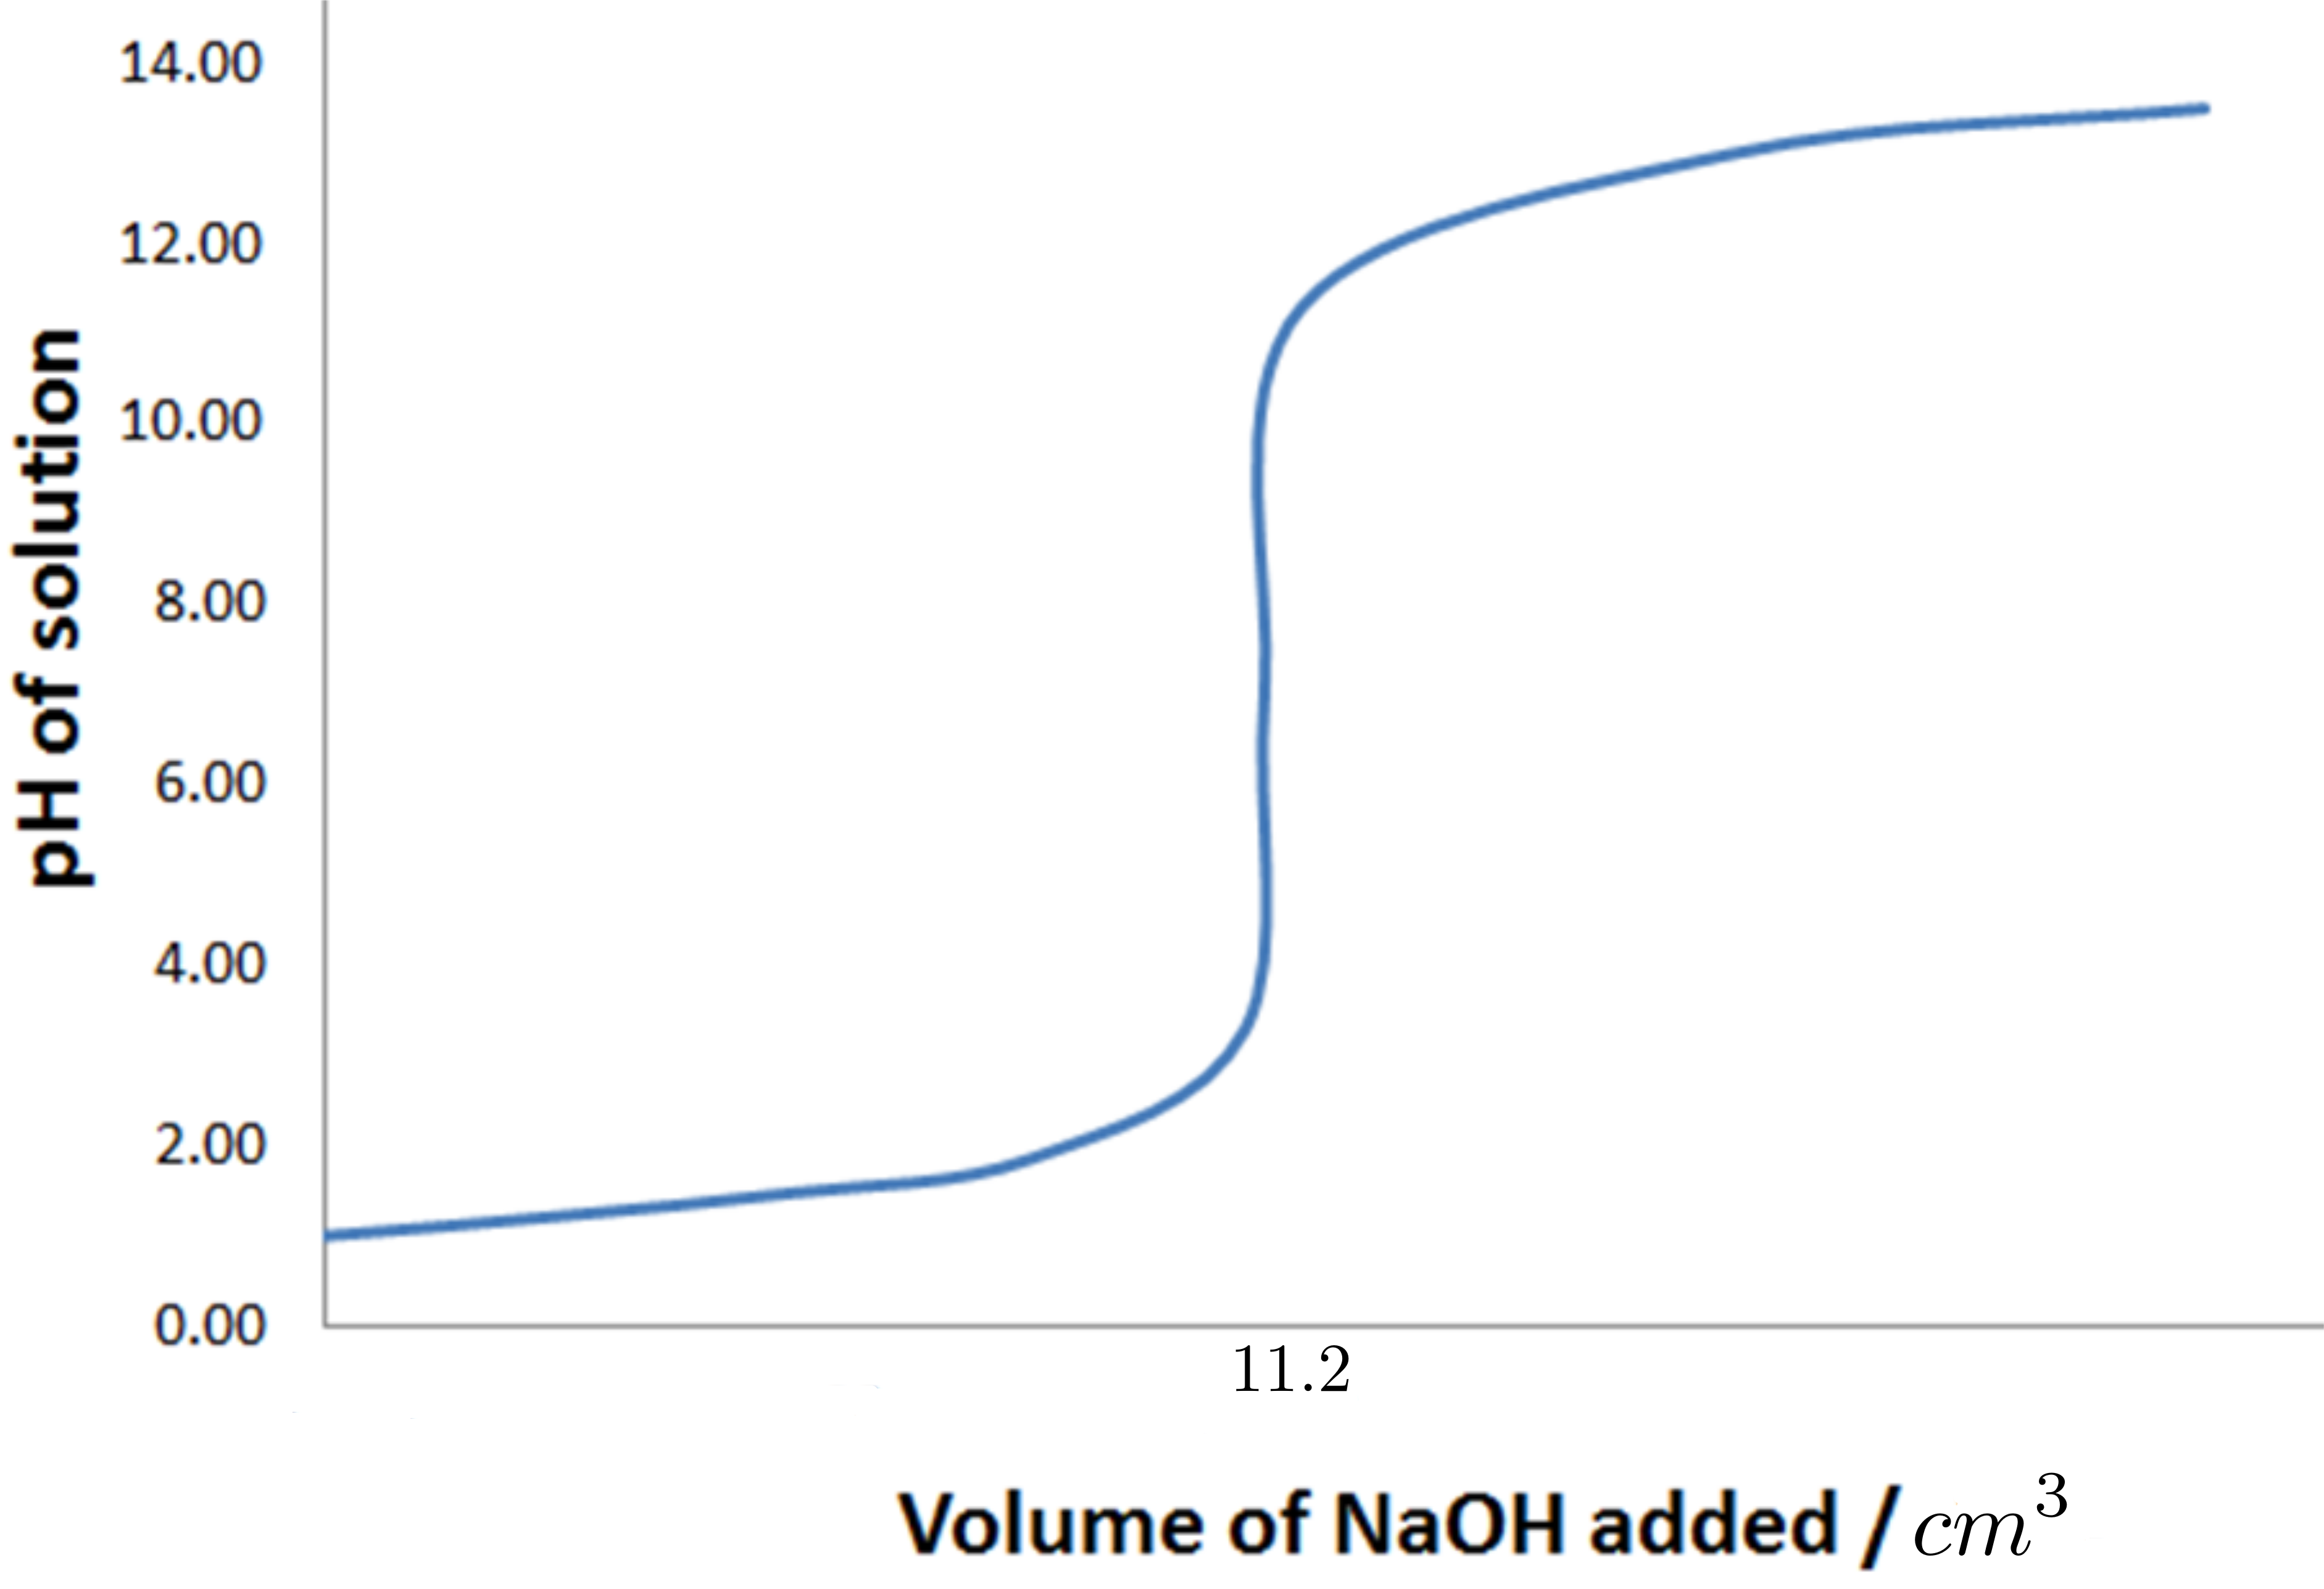
\includegraphics[scale=0.07]{ph_curve}
\hfill
%%%%%%%%%%%%%%%%%%%%%%%%%%%%%%%%%%%%%%%%%%%%%%%%%%%%%%%%%%%%%%%%%%%%%%%%%%
\item[\textbf{ii.}] Visa med hjälp av en uträkning att den initiala koncentrationen av syran är $ 5.62*10^{-2}\ mol/dm^3 $

$ pH=-log([H^+]) $

$ C_{init}(HX)=10^{-1.25}\ =\ 5.62*10^{-2}\ mol/dm^{-3} $

Eftersom syran är stark dissocieras den fullständigt: $ [H^+] = C_{init}(HX) $

\pagebreak

%%%%%%%%%%%%%%%%%%%%%%%%%%%%%%%%%%%%%%%%%%%%%%%%%%%%%%%%%%%%%%%%%%%%%%%%%%
\item[\textbf{iii.}] Beräkna molmassan av syran $ HX $.

$ n=C*V $

$ n(HX)=10^{-1.25}*0.5 = 0.028117\ mol $
\newline
\newline
$ n=\frac{m}{M}\ \rightarrow\ M=\frac{m}{n} $

$ m(HX)=m(Avkalkare)*0.91 $

$ m(HX)=3.00*0.91=2.73\ g $

$ M(HX)=\frac{2.73}{0.028117}=97.0942845965\ g/mol $

\hfill
%%%%%%%%%%%%%%%%%%%%%%%%%%%%%%%%%%%%%%%%%%%%%%%%%%%%%%%%%%%%%%%%%%%%%%%%%%
\item[\textbf{iv.}] Beräkna koncentrationen av $ NaOH(aq) $

$ HX\ +\ NaOH\ \rightarrow\ Na^+\ +\ X^-\ +\ H_2O $

$ n_{init}(HX)=n_{eq}(OH^-) $

$ n_{init}(HX)= 10^{-1.25}*0.02=0.0011247\ mol $

$ n_{eq}(OH^-)\ =\ 1.13*10^{-3}\ mol $

$ C=\frac{n}{V} $

$ C(OH^-)\ =\ \frac{1.13*10^{-3}}{0.0112}\ =\ 0.01\ mol/dm^3 $

\hfill
%%%%%%%%%%%%%%%%%%%%%%%%%%%%%%%%%%%%%%%%%%%%%%%%%%%%%%%%%%%%%%%%%%%%%%%%%%
\item[\textbf{v.}]

\end{itemize}
%%%%%%%%%%%%%%%%%%%%%%%%%%%%%%%%%%%%%%%%%%%%%%%%%%%%%%%%%%%%%%%%%%%%%%%%%%
% End
%%%%%%%%%%%%%%%%%%%%%%%%%%%%%%%%%%%%%%%%%%%%%%%%%%%%%%%%%%%%%%%%%%%%%%%%%%

\end{flushleft}
\end{document}
